\documentclass{article}

\usepackage{xeCJK}
\usepackage{graphicx}
\usepackage{caption}
\usepackage{subfigure}
\usepackage[colorlinks=true,
linkcolor=blue
]{hyperref}
\usepackage{listings}
\usepackage[outputdir=build]{minted}
\usepackage{amsmath}
\usepackage{lastpage}   %获得总页数
\usepackage{fancyhdr}
\usepackage{bookmark}
\graphicspath{{../img/}}
\pagestyle{fancy}
\setlength{\headheight}{64pt}
\lhead{}
\chead{}
\rhead{}
\lfoot{}
\cfoot{}
\rfoot{\thepage\ of \pageref{LastPage}} % 当前页 of 总页数
\renewcommand{\headrulewidth}{0.4pt}    % 改为0pt即可去掉页眉下面的横线
\renewcommand{\footrulewidth}{0.4pt}    % 改为0pt即可去掉页脚上面的横线
\lhead{
\includegraphics[height=0.8in]{depsast.jpg}}  % 插入科协LOGO
\setCJKfamilyfont{yy}{YouYuan}                       % 幼圆  yy

\newcommand{\yy}{\CJKfamily{yy}}
\renewcommand{\baselinestretch}{1.6}

\makeatletter
\renewcommand\paragraph{\@startsection{paragraph}{4}{\z@}%
            {-2.5ex\@plus -1ex \@minus -.25ex}%
            {1.25ex \@plus .25ex}%
            {\normalfont\normalsize\bfseries}}  % make paragraph act like 'subsubsubsection'
\makeatother
\setcounter{secnumdepth}{4} % how many sectioning levels to assign numbers to
\setcounter{tocdepth}{4}    % how many sectioning levels to show in ToC

\graphicspath{{./img/mpu/}{./img/}}

\begin{document}


\title{6-7 MPU6050 运动传感器模块介绍}
\author{工程物理系学生科协技术部\quad 高一川}
\date{\today}
\maketitle
\tableofcontents
\newpage

\section{MPU6050 简介}

MPU6050 是一种非常流行的空间运动传感器芯片,基于 MEMS 技术,它可以获取器件当前的三个加速度分量和三个旋转角速度。由于其体积小巧,功能强大,精度较高,不仅被广泛应用于工业,同时也是航模爱好者的神器,被安装在各类飞行器上驰骋蓝天。在我们的智能车大赛中,它被用于获取智能车转弯时转过的角度,是完成赛道重建,以达到赛题要求必不可少的模块之一。

\section{MPU6050 通讯协议}
\subsection{\texorpdfstring{$I^2C$}{I2C} 协议简介}
MPU6050 与单片机之间的通讯使用 $I^2C$ 协议,这是一种简单的两线制串行通讯协议,下面介绍一下这一协议的基本知识,感兴趣的同学可以访问 \href{http://www.cnblogs.com/hzl6255/p/4298353.html}{http://www.cnblogs.com/hzl6255/p/4298353.html} 了解更多细节。

\subsubsection{物理层简介}
$I^2C$ 总线使用两根信号线 SDA、SCL 与一根地线完成全部数据传输,其中 SDA 指 Serial Data Line,即串行信号线;SCL 指 Serial Clock Line,即串行时钟线。在我们的智能车中,信号均采用 3.3V 电平,同时在信号线悬空时由电阻上拉为高电平。

\subsubsection{信号简介}
在 $I^2C$ 协议中共规定了三种信号,分别是开始信号、结束信号与应答信号。

\begin{figure}[h]
\centering % 使后面的内容居中
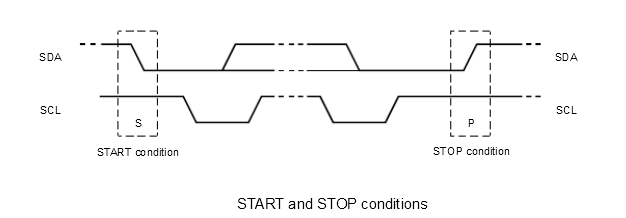
\includegraphics[width=.8\textwidth]{i2c_startstop.png}
\caption{开始信号与结束信号}
\label{i2c_startstop}
\end{figure}

开始信号与结束信号的时序如图 \ref{i2c_startstop}。开始信号指的是 SCL 为高电平时, SDA 由高电平向低电平跳变, 此时总线上开始传送数据;与之相反,结束信号是 SCL 为高电平时, SDA 由低电平向高电平跳变, 结束传送数据。在每次开始或结束数据发送时均要以对应的信号开始。

\begin{figure}[h]
\centering % 使后面的内容居中
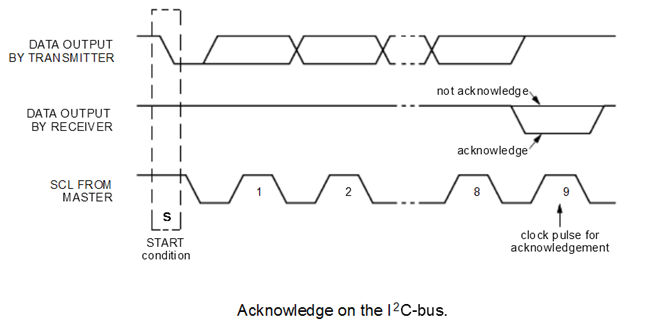
\includegraphics[width=.8\textwidth]{i2c_ack.png}
\caption{应答信号}
\label{i2c_ack}
\end{figure}

应答信号的时序如图 \ref{i2c_ack}。当主机发送完毕 8 位数据,同时被从机正常接收后,从机会在 SDA 线上向主机发送特定的低电平脉冲,此脉冲的存在与否便可以说明信号是否被正常接收。

\subsubsection{地址简介}
$I^2C$ 允许在单总线上连接多个器件。但与 SPI 总线不同的是,$I^2C$ 总线不需要额外的片选线来区分这些器件,而是通过每个器件的不同地址来进行区分。$I^2C$ 协议中规定地址为 8 位,其中高 7 位是从机的地址,最低位表示数据方向(主机读从机数据为1,主机写从机数据为0)。

以 MPU6050 为例,查看它的数据手册,你会发现在 \lstinline{Electrical Specifications} 这一表格中有一栏为 \lstinline{I2C ADDRESS},其值为 1101000 或者 1101001。那么同一款芯片,为什么会有多个地址呢?让我们从芯片的引脚说起。

在每款使用 $I^2C$ 总线通讯的芯片上,通常都会有 1 到多个标注为 ADx 的引脚,它们便是这款芯片的地址设置引脚。我们已经知道了地址一共有 7 位,但芯片上的引脚有限,不可能使用 7 个引脚来设置整个地址,那么聪明的芯片厂商就选择了通过少数几根线来设置地址的其中几位,以区分单总线上的同款芯片。同样还是以 MPU6050 为例,它只有一个地址设置引脚为 AD0,根据数据手册可以知道它的高低电平决定了 7 位地址的最后一位。这样,我们便可以在同一个 $I^2C$ 总线上连接两个 MPU6050。在智能车的原理图中,这一地址线被接地了,那么聪明的你一定会想到他的地址是 0x68(1101000)。

\subsubsection{数据传输过程}

\begin{figure}[h]
\centering % 使后面的内容居中
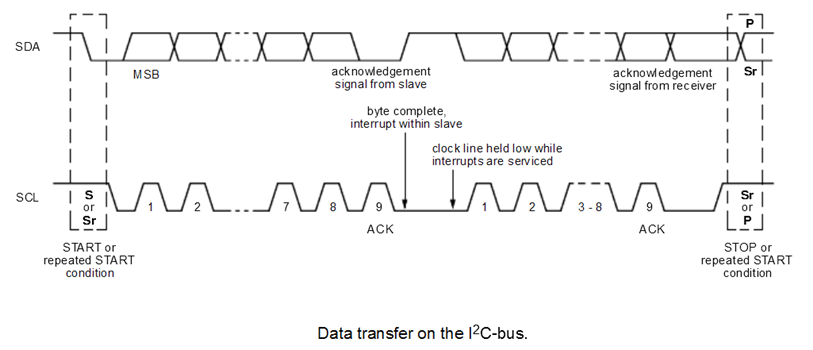
\includegraphics[width=.8\textwidth]{i2c_timing.png}
\caption{应答信号}
\label{i2c_timing}
\end{figure}

$I^2C$ 协议的数据传输以字节为单位,首先传输最高位 MSB。在每个字节传输后,均需要从机发送应答信号。每次传输的时序如图 \ref{i2c_timing} 所示。每次传输的第一个字节均是前面描述过的 8 位地址,在收到从机应答后继续发送其余数据,每次传输的数据量不受限制。

\subsection{MPU6050 通讯代码}
本章将结合拉普兰德底层库中 \lstinline{DEV_MPU6050} 的具体实现,来讲解 MPU6050 与单片机的通讯协议。注意在这里我们使用了 K60 芯片的硬件 $I^2C$ 模块,所以不会涉及到具体的时序。

\subsubsection{从 MPU6050 读出数据}
在一般的传感器中,我们所需要的数据都存储在传感器芯片内的寄存器中。寄存器是芯片内一块特殊的存储区域,通常每个寄存器可以存储 8 位二进制数,同时以其自身的一个 8 位二进制地址来标识。每个寄存器都具有其特定的功能,其具体功能可以通过查阅芯片数据手册来得知。其代码实现如下:

\begin{minted}[showspaces=false,breaklines=true]{c}

uint8 MPU6050_ReadReg(uint8 RegisterAddress) {
  uint8 result;

  // 开始本次传输并发送从机地址
  LPLD_I2C_StartTrans(MPU6050_I2CX, SlaveAddress, I2C_MWSR);
  LPLD_I2C_WaitAck(MPU6050_I2CX, I2C_ACK_ON);

  // 写 MPU6050 寄存器地址,告知芯片所要读取的寄存器地址
  LPLD_I2C_WriteByte(MPU6050_I2CX, RegisterAddress);
  LPLD_I2C_WaitAck(MPU6050_I2CX, I2C_ACK_ON);

  // 再次产生开始信号,以开始读取数据
  LPLD_I2C_ReStart(MPU6050_I2CX);

  // 发送从机地址,并设置 R/W 位为 1 以开始读取
  LPLD_I2C_WriteByte(MPU6050_I2CX, (SlaveAddress<<1)|I2C_MRSW);
  LPLD_I2C_WaitAck(MPU6050_I2CX, I2C_ACK_ON);

  // 转换主机模式为读(硬件库所需)
  LPLD_I2C_SetMasterWR(MPU6050_I2CX, I2C_MRSW);

  // 关闭应答 ACK
  LPLD_I2C_WaitAck(MPU6050_I2CX, I2C_ACK_OFF);//关闭ACK

  // 读 I2C 数据
  result = LPLD_I2C_ReadByte(MPU6050_I2CX);
  LPLD_I2C_WaitAck(MPU6050_I2CX, I2C_ACK_ON);

  // 发送停止信号,结束本次传输
  LPLD_I2C_Stop(MPU6050_I2CX);

  // 再次读取 I2C 数据,保证读取的数据完整
  result = LPLD_I2C_ReadByte(MPU6050_I2CX);

  LPLD_SYSTICK_DelayMs(1);
  return result;
}

\end{minted}

\subsubsection{向 MPU6050 写入数据}
向 MPU6050 中写入数据比读取简单得多,代码如下:

\begin{minted}[showspaces=false,breaklines=true]{c}

void MPU6050_WriteReg(uint8 RegisterAddress, uint8 Data) {
  // 开始本次传输并发送从机地址
  LPLD_I2C_StartTrans(MPU6050_I2CX, SlaveAddress, I2C_MWSR);
  LPLD_I2C_WaitAck(MPU6050_I2CX, I2C_ACK_ON);  // 等待应答

  // 发送 MPU6050 寄存器地址
  LPLD_I2C_WriteByte(MPU6050_I2CX, RegisterAddress);
  LPLD_I2C_WaitAck(MPU6050_I2CX, I2C_ACK_ON);

  // 向寄存器中写具体数据
  LPLD_I2C_WriteByte(MPU6050_I2CX, Data);
  LPLD_I2C_WaitAck(MPU6050_I2CX, I2C_ACK_ON);

  LPLD_I2C_Stop(MPU6050_I2CX);
}

\end{minted}

\subsection{MPU6050 数据格式}
\subsubsection{寄存器表}
对于运动传感器,我们关心的数据都存储在地址为 0x3B 到 0x48 这几个寄存器中,共有 14 个寄存器,其中存储了 7 个不同的数据,每个数据均为 16 位,占用两个寄存器。寄存器地址与数据名称的对应关系如表 \ref{mpu_regs}。

\begin{table}[htbp]
 \centering
 \caption{MPU6050 寄存器表}
 \label{mpu_regs}
 \begin{tabular}{|l|l|l|}
  \hline
  寄存器地址 & 寄存器名称 & 数据名称         \\ \hline
  0x3B     & ACC\_X    & 加速度 X 轴分量    \\
  0x3D     & ACC\_Y    & 加速度 Y 轴分量    \\
  0x3F     & ACC\_Z    & 加速度 Z 轴分量    \\
  0x41     & TEMP     & 环境温度          \\
  0x43     & GYR\_X    & 陀螺仪 X 轴分量    \\
  0x45     & GYR\_Y    & 陀螺仪 Y 轴分量    \\
  0x47     & GYR\_Z    & 陀螺仪 Z 轴分量    \\ \hline
 \end{tabular}
\end{table}

\subsubsection{芯片坐标系定义}

\begin{figure}[h]
\centering % 使后面的内容居中
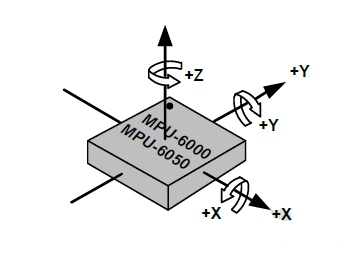
\includegraphics[width=.4\textwidth]{mpu_axis.jpg}
\caption{MPU6050 三轴方向}
\label{mpu_axis}
\end{figure}

MPU6050 芯片自身的坐标系是这样定义的:令芯片表面朝向自己,将其表面文字转至正确角度,此时,以芯片内部中心为原点,水平向右的为 X 轴,向前的为 Y 轴,垂直向上的为 Z 轴。在智能车的 PCB 上,MPU6050 芯片的位置为 PCB 横向的中心,同时为了布线方便,对芯片进行了旋转,所以在智能车上的坐标系定义为:以芯片内部中心(小车横向中心)为原点,小车前进方向为 X 轴正方向,左侧为 Y 轴正方向,竖直向上的方向为 Z 轴正方向。三轴角速度的正方向可以参考图 \ref{mpu_axis}。

\subsubsection{物理量解释及数据格式}
\paragraph{加速度计}
加速度计的三轴分量 ACC\_X、ACC\_Y 和 ACC\_Z 均为 16 位有符号整数,分别表示器件在三个轴向上的加速度,取负值时加速度沿坐标轴负向,取正值时沿正向。

三个加速度分量均以重力加速度 g 的倍数为单位,能够表示的加速度范围,即倍率可以统一设定,有 4 个可选倍率:2g、4g、8g、16g。以 ACC\_X 为例,若倍率设定为 2g(默认),则意味着 ACC\_X 取最大值 32767 时,当前加速度为沿 X 轴正方向 2 倍的重力加速度;若设定为 4g,取 32767 时表示沿 X 轴正方向 4 倍的重力加速度,以此类推。显然,倍率越低精度越好,倍率越高表示的范围越大,这要根据具体的应用来设定。在智能车大赛提供的代码中,这一倍率被设置为了 2g,如果需要修改,请改动 \lstinline{DEV_MPU6050.h} 中的有关宏定义。

三轴加速度值寄存器值与加速度的换算公式为:$a_x=4g*ACC\_X/32768$(g 为当地重力加速度)。

\paragraph{陀螺仪}
陀螺仪输出的数据为小车绕 X、Y 和 Z 三个坐标轴旋转的角速度分量 GYR\_X、GYR\_Y 和 GYR\_Z。它们均为 16 位有符号整数。从原点向旋转轴方向看去,取正值时为顺时针旋转,取负值时为逆时针旋转。

三个角速度分量均以“度/秒”为单位,能够表示的角速度范围,即倍率可统一设定,有4个可选倍率:250度/秒、500度/秒、1000度/秒、2000度/秒。以 GYR\_X 为例,若倍率设定为 250 度/秒,则意味着 GYR\_X 取正最大值 32767 时,当前角速度为顺时针 250 度/秒;若设定为 500 度/秒,取 32767 时表示当前角速度为顺时针 500 度/秒。显然,倍率越低精度越好,倍率越高表示的范围越大。在代码中,这一倍率被设置为了 2000 度/秒。

三轴陀螺仪寄存器值与角速度的换算公式为:$\omega_x=2000*GYR\_X/32768$。

\paragraph{温度}
MPU6050 中有一个内置的温度传感器,其读出的寄存器值与温度(摄氏度)的换算公式为:$T=TEMP/340+36.53$。

\section{MPU6050 数据处理}
\subsection{积分处理}
在智能车大赛的赛题要求中,需要我们进行赛道图像的重建,那么就需要获得赛道每条直线的长度信息以及每个弯道处的转弯角度信息。长度信息可以使用编码器进行获取,而转角信息就需要使用 MPU6050 中的陀螺仪数据进行获取。陀螺仪输出的数据为角速度,要转换为转弯角度,就需要对其关于时间进行积分处理。在积分时,我们关心的是 Z 轴的数值,于是需要使用单片机内的定时器进行操作,在转弯开始时开启定时器,由定时器中断每隔固定的时间间隔读取 Z 轴的陀螺仪输出数值,并将时间间隔与该值相乘,不断累加直到转弯结束,便可以得知本次转弯转过的总角度。这一部分的代码并不复杂,你可以尝试自己使用我们提供的定时器有关函数进行编写。

\subsection{滤波处理}
MPU6050 作为一款 MEMS 传感器,其灵敏度很高,但同时数据中所含的噪声也很多,在使用时就需要进行恰当的滤波处理。在我们提供的代码中,已经开启了芯片内置的滤波器模块,对数据进行了简单的过滤处理。如果你对这一滤波效果不满意的话,可以参考网络上的各种资料,引入滑动平均滤波法或者卡尔曼滤波算法进行进一步的滤波处理。

\section{MPU6050 编程指南}
为便于数据的读取,我们对寄存器读取以及数据单位的转换代码进行了封装,并使用 \lstinline{MPU6050_result} 结构体存储传感器读取结果。这一结构体的定义为:

\begin{minted}[showspaces=false,breaklines=true]{c}

typedef struct {

  double accel_x,accel_y,accel_z; // 三轴加速度值 (m/s^2)
  double gyro_x,gyro_y,gyro_z;    // 三轴陀螺仪角速度 (deg/s)
  float32 temperature;  // 温度

} MPU6050_result;

\end{minted}

同时我们提供了 \lstinline{MPU6050_read()} 函数,在需要读取 MPU6050 的数据时,只需调用该函数即可。该函数代码为:

\begin{minted}[showspaces=false,breaklines=true]{c}

MPU6050_result MPU6050_read() {
  MPU6050_result ret;   // 临时结构体

  ret.accel_x = MPU6050_GetResult(ACCEL_XOUT_H)/32767.0*2.0*GRAVITY;  // X 加速度
  ret.accel_y = MPU6050_GetResult(ACCEL_YOUT_H)/32767.0*2.0*GRAVITY;  // Y 加速度
  ret.accel_z = MPU6050_GetResult(ACCEL_ZOUT_H)/32767.0*2.0*GRAVITY;  // Z 加速度

  ret.gyro_x  = MPU6050_GetResult(GYRO_XOUT_H)/2000.0;  // X 陀螺仪
  ret.gyro_y  = MPU6050_GetResult(GYRO_YOUT_H)/2000.0;  // Y 陀螺仪
  ret.gyro_z  = MPU6050_GetResult(GYRO_ZOUT_H)/2000.0;  // Z 陀螺仪

  ret.temperature = MPU6050_GetResult(TEMP_OUT_H)/340+36.53;  // 温度

  return ret;
}

\end{minted}

\end{document}
